%# -*- coding: utf-8-unix -*-
%%==================================================
%% chapter01.tex for SJTU Master Thesis
%%==================================================

%\bibliographystyle{sjtu2}%[此处用于每章都生产参考文献]
\chapter{系统测试}
\label{chap:sys_test}

qscache系统的测试工作由测试目标与测试方法、qscache系统性能测试、qscache系统对I/O带宽按权限分配的测试三个部分组成,接下来将分别进行介绍。

\section{测试目标与测试方法}

\subsection{测试目标}

测试目标就是要检验所设计的qscache系统是否能达到预期的设计目标,即大容量、低成本、高顺序读写性能、高随机读写性能、多缓存设备对多后台设备的支持、支持I/O带宽按权限分配。

qscache系统中,缓存设备与后台设备作为Device Mapper的target device被加载到系统中,qscache系统的容量取决于被加载的后台设备的容量。只要系统能支持多缓存设备、多后台设备,那么qscache系统就能以多块HDD作为后台设备提供大存储容量。在qscache系统中,缓存设备的容量一般取后台设备的十分之一到八分之一,对于1TB的HDD作为后台设备,取128G的SSD作为缓存设备,系统的成本还是可接受的。因此,测试的内容主要落在qscache系统的性能上以及qscache系统是否支持I/O带宽按权限分配,需要对qscache系统的顺序读写性能与随机读写性能进行测试,验证是否达到预计目标。另外需要开启多个进程设置不同权限,验证不同进程被分配到的I/O带宽是否按权限分配。

\subsection{测试方法}

综合qscache的测试目标,本研究对qscache的性能测试主要采用对比的方法,对比的系统包括:基于HDD的存储系统、开源混合存储系统flashcache、本系统qscache。对于qscache是否支持I/O带宽按权限分配,本研究采用普通的测试方法,通过开启多个测试进程,为不同测试进程设置不同权限,查看不同测试进程最后给出的性能统计进行验证。

\section{测试环境}

测试环境如表\ref{tab:qscache_test_environment}所示

\begin{table}[H]
    \centering
    \bicaption[tab:qscache_test_environment]{qscache性能测试环境}{qscache性能测试环境}{Table}{test environment of qscache}
    \begin{tabular}{cc} \toprule
      机器类型 & 普通台式机 \\ \midrule
      CPU & 单核AMD CPU\\
      内存 & 1GB DDR3\\
      SSD & 120GB intel350 \\
      HDD & WD 1TB 7200rpm绿盘\\
      内核版本 & 3.10.108\\
      \bottomrule
    \end{tabular}
\end{table}

\section{qscache性能测试}

\subsection{系统初始化}

假设Linux系统中,120GB的SSD为/dev/sdb,1TB的HDD为/dev/sdi。首先对Linux内核进行修改、编译、安装,然后对三个系统分别编译安装,首先对第一个系统进行初始化测试,然后当前一个系统的测试完成后,后一个系统才进行初始化与测试。

对内核修改后,内核的编译安装过程如下:

\begin{enumerate}
    \item cp /boot/config-3.10.0-693.5.2.el7.x86\_64 .config
    \item 在系统原有的内核配置文件的基础上建立新的编译选项:sh -c \lq yes \lq\lq\rq\rq | make oldconfig \rq
    \item 生成内核文件:make bzImage
    \item 编译模块:make modules
    \item 编译安装模块:make modules\_install
    \item 安装:make install
    \item reboot加载新内核
\end{enumerate}

四个系统的初始化操作如下:

\begin{enumerate}
    \item 基于HDD系统的初始化
          \begin{enumerate}
              \item 格式化文件系统为ext4:mkfs.ext4 /dev/sdi
          \end{enumerate}
    \item flashcache的初始化
    \begin{enumerate}
        \item 编译,需要内核的源码树:make KERNEL\_TREE=/usr/src/linux-3.10.108/
        \item 加载:insmod src/flashcache.ko
        \item 以写回模式创建混合存储系统,缓存设备容量120GB,后台设备容量1TB,mapped device命名为cachedev:flashcache\_create -p back cachedev /dev/sdb /dev/sdi
        \item 格式化文件系统为ext4:mkfs.ext4 /dev/mapper/cachedev
    \end{enumerate}
    \item 基于bio的qscache的初始化
    \begin{enumerate}
        \item 编译,需要内核的源码树:make KERNEL\_TREE=/usr/src/linux-3.10.108/
        \item 加载,以基于request的模式加载:insmod src/qscache.ko request\_based=0
        \item 以写回模式创建混合存储系统,缓存设备容量120GB,后台设备容量1TB,mapped device命名为cachedev:qscache\_create -p back -n cachedev -c /dev/sdb -h /dev/sdi
        \item 格式化文件系统为ext4:mkfs.ext4 /dev/mapper/cachedev
    \end{enumerate}
    \item 基于request的qscache的初始化
    \begin{enumerate}
        \item 编译,需要内核的源码树:make KERNEL\_TREE=/usr/src/linux-3.10.108/
        \item 加载,以基于request的模式加载:insmod src/qscache.ko request\_based=1
        \item 以写回模式创建混合存储系统,缓存设备容量120GB,后台设备容量1TB,mapped device命名为cachedev:qscache\_create -p back -n cachedev -c /dev/sdb -h /dev/sdi
        \item 格式化文件系统为ext4:mkfs.ext4 /dev/mapper/cachedev
    \end{enumerate}
\end{enumerate}

\subsection{顺序读写性能对比}

顺序读写性能使用fio进行对比测试,文件大小为4GB,块大小从4KB到16MB,命令为fio -filename=/dev/mapper/cachedev -direct=1 -iodepth1 -thread -rw=RW -ioengine=libaio -bs=BS -size=4G -numjobs=8 -runtime=30 -name=readtest,通过设置BS来设置块大小,通过设置RW为read或write来设置顺序读或顺序写。顺序读写性能测试结果如表\ref{tab:seq_comparison}所示。

\begin{table}[!ht]
    \centering
    \bicaption[tab:seq_comparison]{HDD、flashcache、qscache顺序读写性能}{HDD、flashcache、qscache顺序读写性能(KB/s)}{Table}{comparison of sequential performance among HDD, flashcache and qscache(KB/s)}
    \begin{tabular}{@{}ccccccccc@{}} 
      \toprule
      \multirow{2}*{块大小} & \multicolumn{2}{c}{HDD} & \multicolumn{2}{c}{flashcache} & \multicolumn{2}{c}{bio-qscache} & \multicolumn{2}{c}{request-qscache}\\
      & read & write & read & write & read & write & read & write\\
      \midrule
      4KB & 203686 & 202350 & 184067 & 113235 & 184395 & 110970 & 175886 & 106754\\
      8KB & 211129 & 229899 & 187215 & 135352 & 181659 & 125204 & 173932 & 110897\\
      16KB & 196616 & 203539 & 171163 & 128776 & 172225 & 116473 & 164517 & 114719\\
      32KB & 190884 & 194822 & 159974 & 131076 & 162917 & 115747 & 160245 & 104128\\
      64KB & 184689 & 181444 & 153915 & 141162 & 166891 & 115823 & 164157 & 110325\\
      128KB & 208728 & 214504 & 181982 & 145134 & 164893 & 118921 & 137718 & 106245\\
      256KB & 222185 & 200914 & 189187 & 127656 & 189762 & 105847 & 167462 & 103723\\
      512KB & 229497 & 193496 & 187896 & 105086 & 198944 & 118349 & 156784 & 105581\\
      1MB & 204723 & 211884 & 173823 & 126227 & 164305 & 115985 & 157783 & 102373\\
      2MB & 208785 & 201776 & 187231 & 124686 & 177806 & 115864 & 167256 & 108699\\
      4MB & 261920 & 260618 & 196758 & 125859 & 185505 & 116010 & 165823 & 101882\\
      8MB & 232480 & 220825 & 206443 & 134810 & 199202 & 104759 & 186614 & 94646\\
      16MB & 234581 & 210528 & 201457 & 122041 & 191742 & 113412 & 189106 & 105182\\
      \bottomrule
    \end{tabular}
\end{table}

四者的顺序读性能对比如图\ref{fig:seq_read_comparison}所示,可以看到基于HDD的系统的吞吐量能达到220MB/s,而flashcache大约为170MB/s,基于bio的qscache和flashcache差不多也在170MB/s左右,而基于request的qscache大约为160MB/s。这是因为,对于基于HDD的系统而言,读请求直接从HDD上读取数据,不需要经历额外步骤;对于flashcache,当设置也缓存顺序操作时,需要先访问SSD查询缓存是否命中,如果未命中还需要去HDD中读取数据并可能会替换缓存,因此额外开销较多;对于基于bio的qscache,由于总体设计和策略与flashcache差不多,因此性能相近;对于基于request的qscache,由于将原本立刻提交的bio请求延缓放入request中,因此性能有所下降。

\begin{figure}[H]
    \centering
    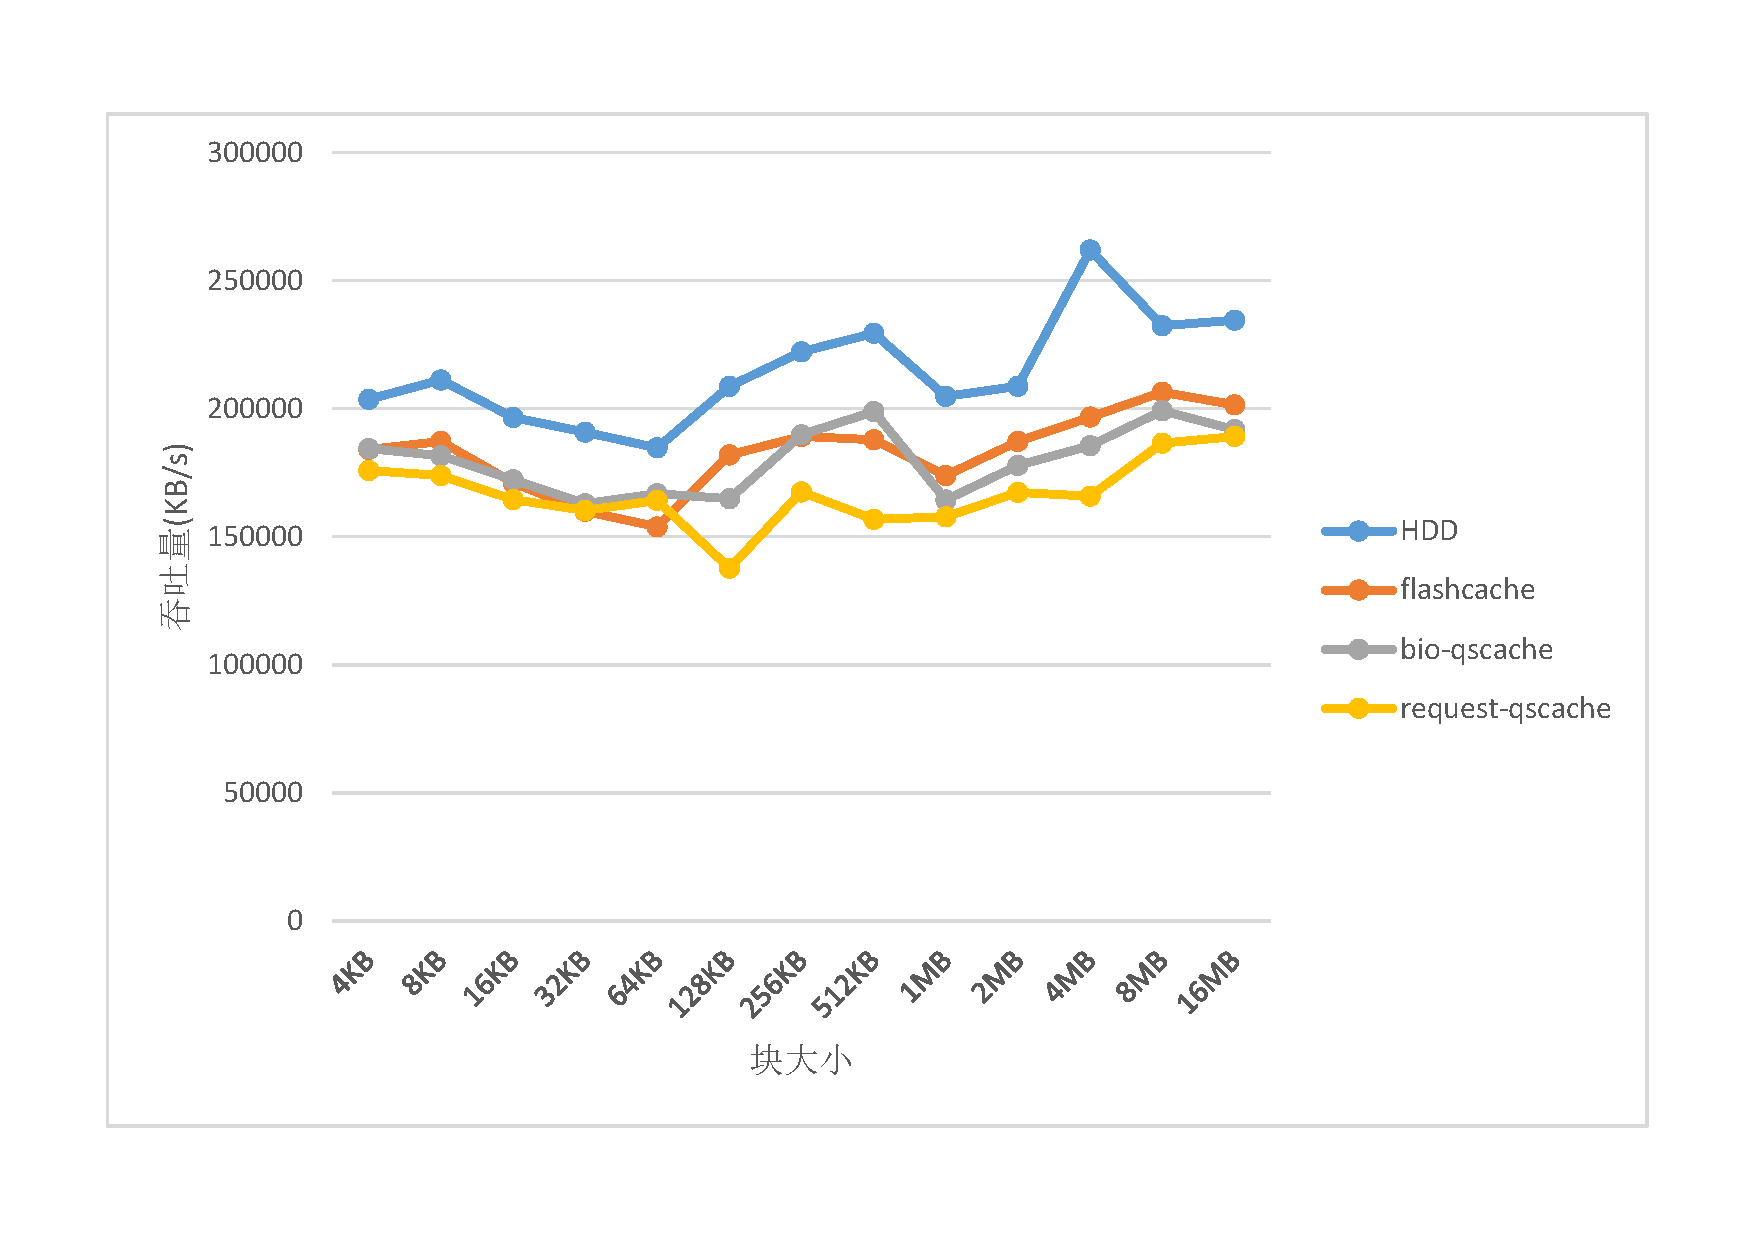
\includegraphics[width=0.8\textwidth]{seq_read.pdf}
    \bicaption[fig:seq_read_comparison]{HDD、flashcache、qscache顺序读性能对比图}{HDD、flashcache、qscache顺序读性能对比图}{Fig.}{comparison of sequential read among HDD, flashcache and qscache}
\end{figure}

四者的顺序写性能对比如图\ref{fig:seq_write_comparison}所示,可以看到基于HDD的系统的吞吐量能达到200MB/s,而flashcache大约为130MB/s,基于bio的qscache差不多在110MB/s左右,而基于request的qscache和基于bio差不多,大约为110MB/s。这是因为,对于基于HDD的系统而言,写请求直接向HDD上写数据,不需要经历额外步骤;对于flashcache,当设置也缓存顺序操作时,需要先访问SSD查询缓存是否命中,如果未命中还需要去HDD中读取数据并可能会替换缓存,然后对缓存中的数据进行更改,并会发生写回,因此额外开销较多;对于基于bio的qscache,由于总体设计和策略与flashcache差不多,因此性能相差不多;对于基于request的qscache,由于将原本立刻提交的bio请求延缓放入request中,因此性能有所下降。

\begin{figure}[H]
    \centering
    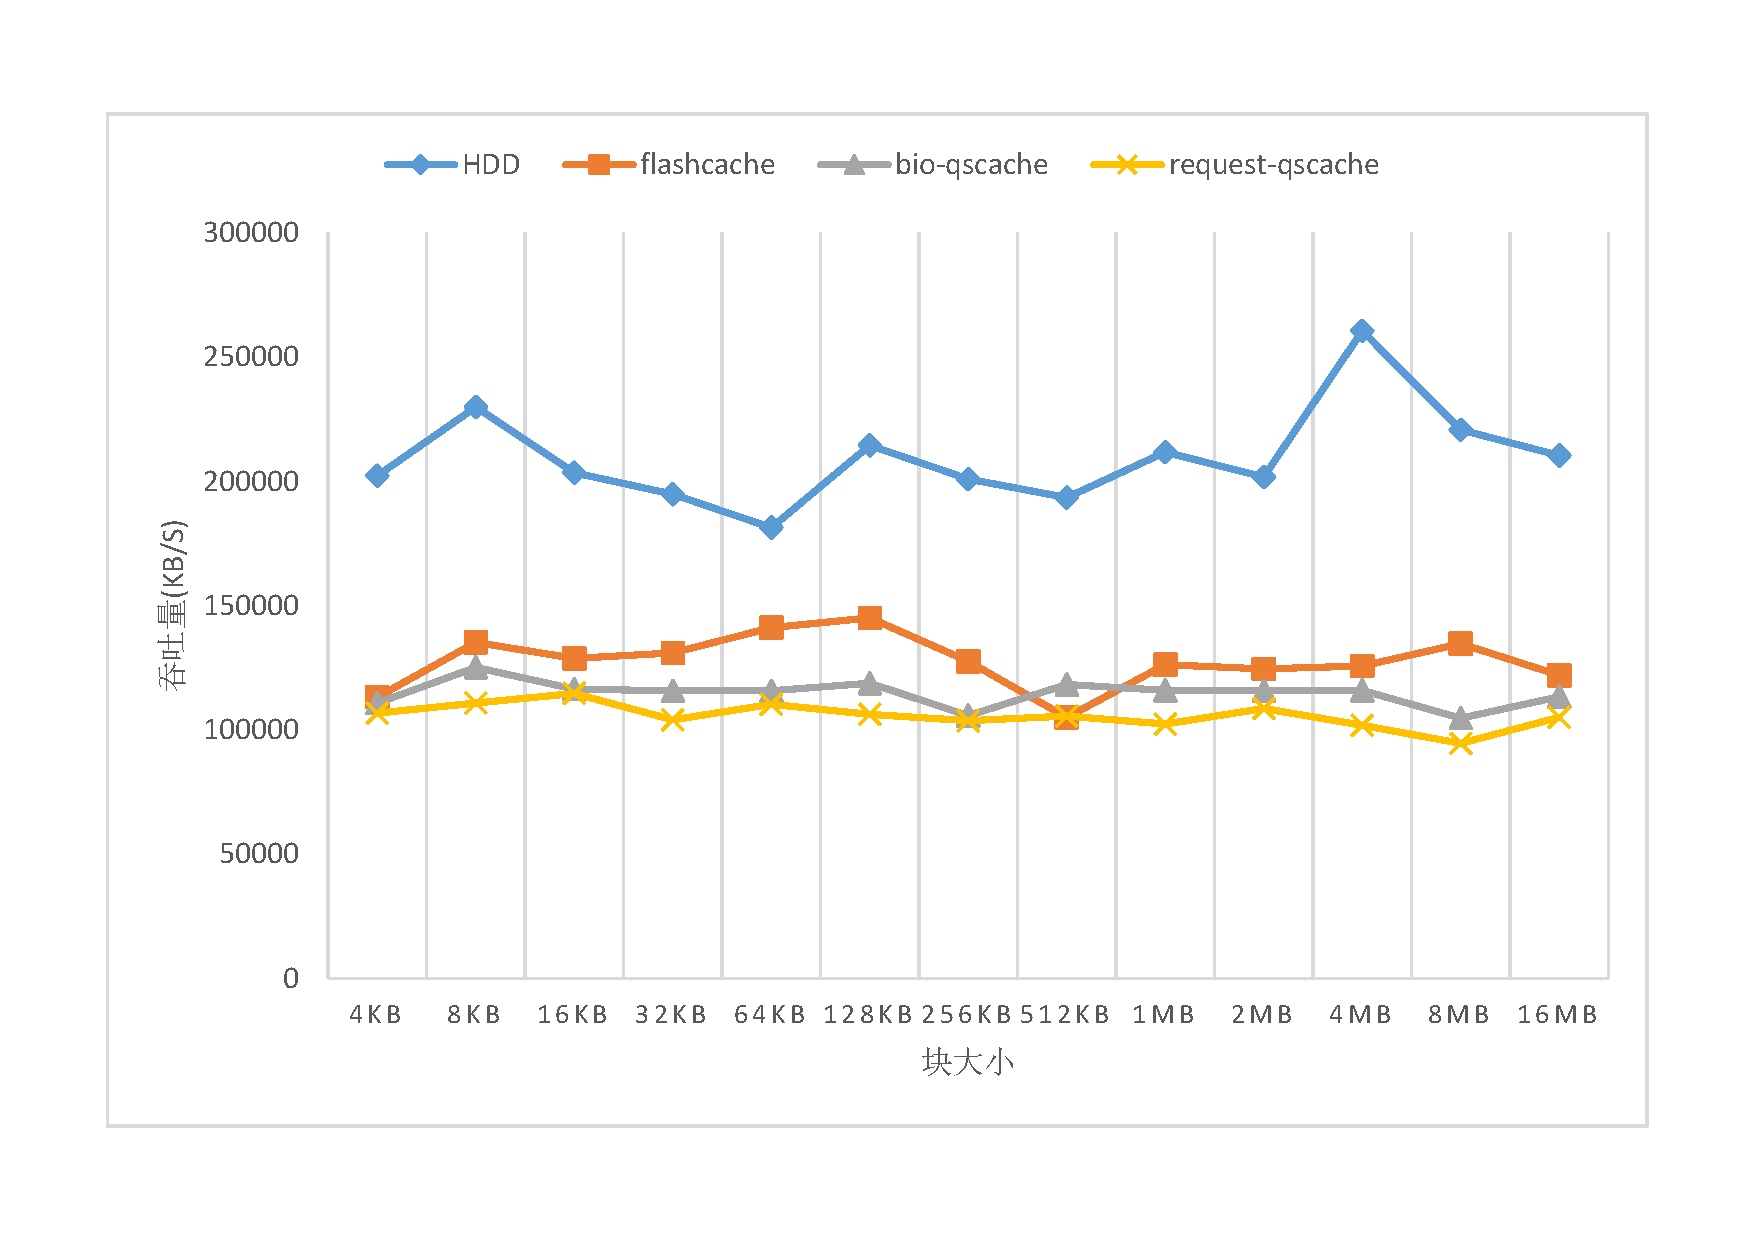
\includegraphics[width=0.8\textwidth]{seq_write.pdf}
    \bicaption[fig:seq_write_comparison]{HDD、flashcache、qscache顺序写性能对比图}{HDD、flashcache、qscache顺序写性能对比图}{Fig.}{comparison of sequential write among HDD, flashcache and qscache}
\end{figure}

\subsection{随机读写性能对比}

随机读写性能使用fio进行对比测试,文件大小为4GB,块大小从4KB到16MB,命令为fio -filename=/dev/mapper/cachedev -direct=1 -iodepth1 -thread -rw=RW -ioengine=libaio -bs=BS -size=4G -numjobs=8 -runtime=30 -name=readtest,通过设置BS来设置块大小,通过设置RW为randread、randwrite或randrw来设置随机读、随机写或混合随机读写。随机读写性能测试结果如表\ref{tab:rand_comparison_1}及表\ref{tab:rand_comparison_2}所示。

\begin{table}[H]
    \centering
    \bicaption[tab:rand_comparison_1]{HDD、flashcache、qscache随机读写性能}{HDD、flashcache、qscache随机读写性能(IOPS)}{Table}{comparison of random performance among HDD, flashcache and qscache(IOPS)}
    \begin{tabular}{@{}ccccccccc@{}} 
      \toprule
      \multirow{2}*{块大小} & \multicolumn{3}{c}{HDD} & \multicolumn{3}{c}{flashcache} \\
      & read & write & read(70\%)/write(30\%) & read & write & read(70\%)/write(30\%)\\
      \midrule
      4KB & 247 & 226 & 143/152 & 21203 & 10843 & 8028/3438\\
      8KB & 213 & 232 & 135/147 & 11277 & 11673 & 6681/2863\\
      16KB & 223 & 227 & 141/144 & 8224 & 10854 & 4727/2030\\
      32KB & 207 & 211 & 135/143 & 4227 & 8949 & 3417/1464\\
      \bottomrule
    \end{tabular}
\end{table}

\begin{table}[H]
    \centering
    \bicaption[tab:rand_comparison_2]{HDD、flashcache、qscache随机读写性能(续)}{HDD、flashcache、qscache随机读写性能(IOPS)(续)}{Table}{comparison of random performance among HDD, flashcache and qscache(IOPS)(continued)}
    \begin{tabular}{@{}ccccccccc@{}} 
      \toprule
      \multirow{2}*{块大小} & \multicolumn{3}{c}{bio-qscache} & \multicolumn{3}{c}{request-qscache}\\
      & read & write & read(70\%)/write(30\%) & read & write & read(70\%)/write(30\%)\\
      \midrule
      4KB & 11812 & 11227 & 7368/3153 & 13649 & 13123 & 8428/3607\\
      8KB & 10286 & 9913 & 6169/2644 & 14251 & 9312 & 6317/2709\\
      16KB & 6284 & 8692 & 4869/2090 & 8929 & 7140 & 4347/1868\\
      32KB & 4650 & 8498 & 3320/1423 & 5785 & 4925 & 2693/1152\\
      \bottomrule
    \end{tabular}
\end{table}


四者的随机读性能对比如图\ref{fig:rand_read_comparison}所示,随机写性能对比如图\ref{fig:rand_write_comparison}所示,可以看到机遇HDD的系统在随机读写方面性能极差,IOPS大约只有200-300,而flashcache和基于bio的qscache以及基于request的qscache的IOPS大约在5000到15000,总的来说flashcache和基于bio的qscache和基于request的qscache在随机读方面性能比较相近,而在随机写方面flashcache和基于bio的qscache性能相近而基于request的qscache性能则较差。

\begin{figure}[!htbp]
    \centering
    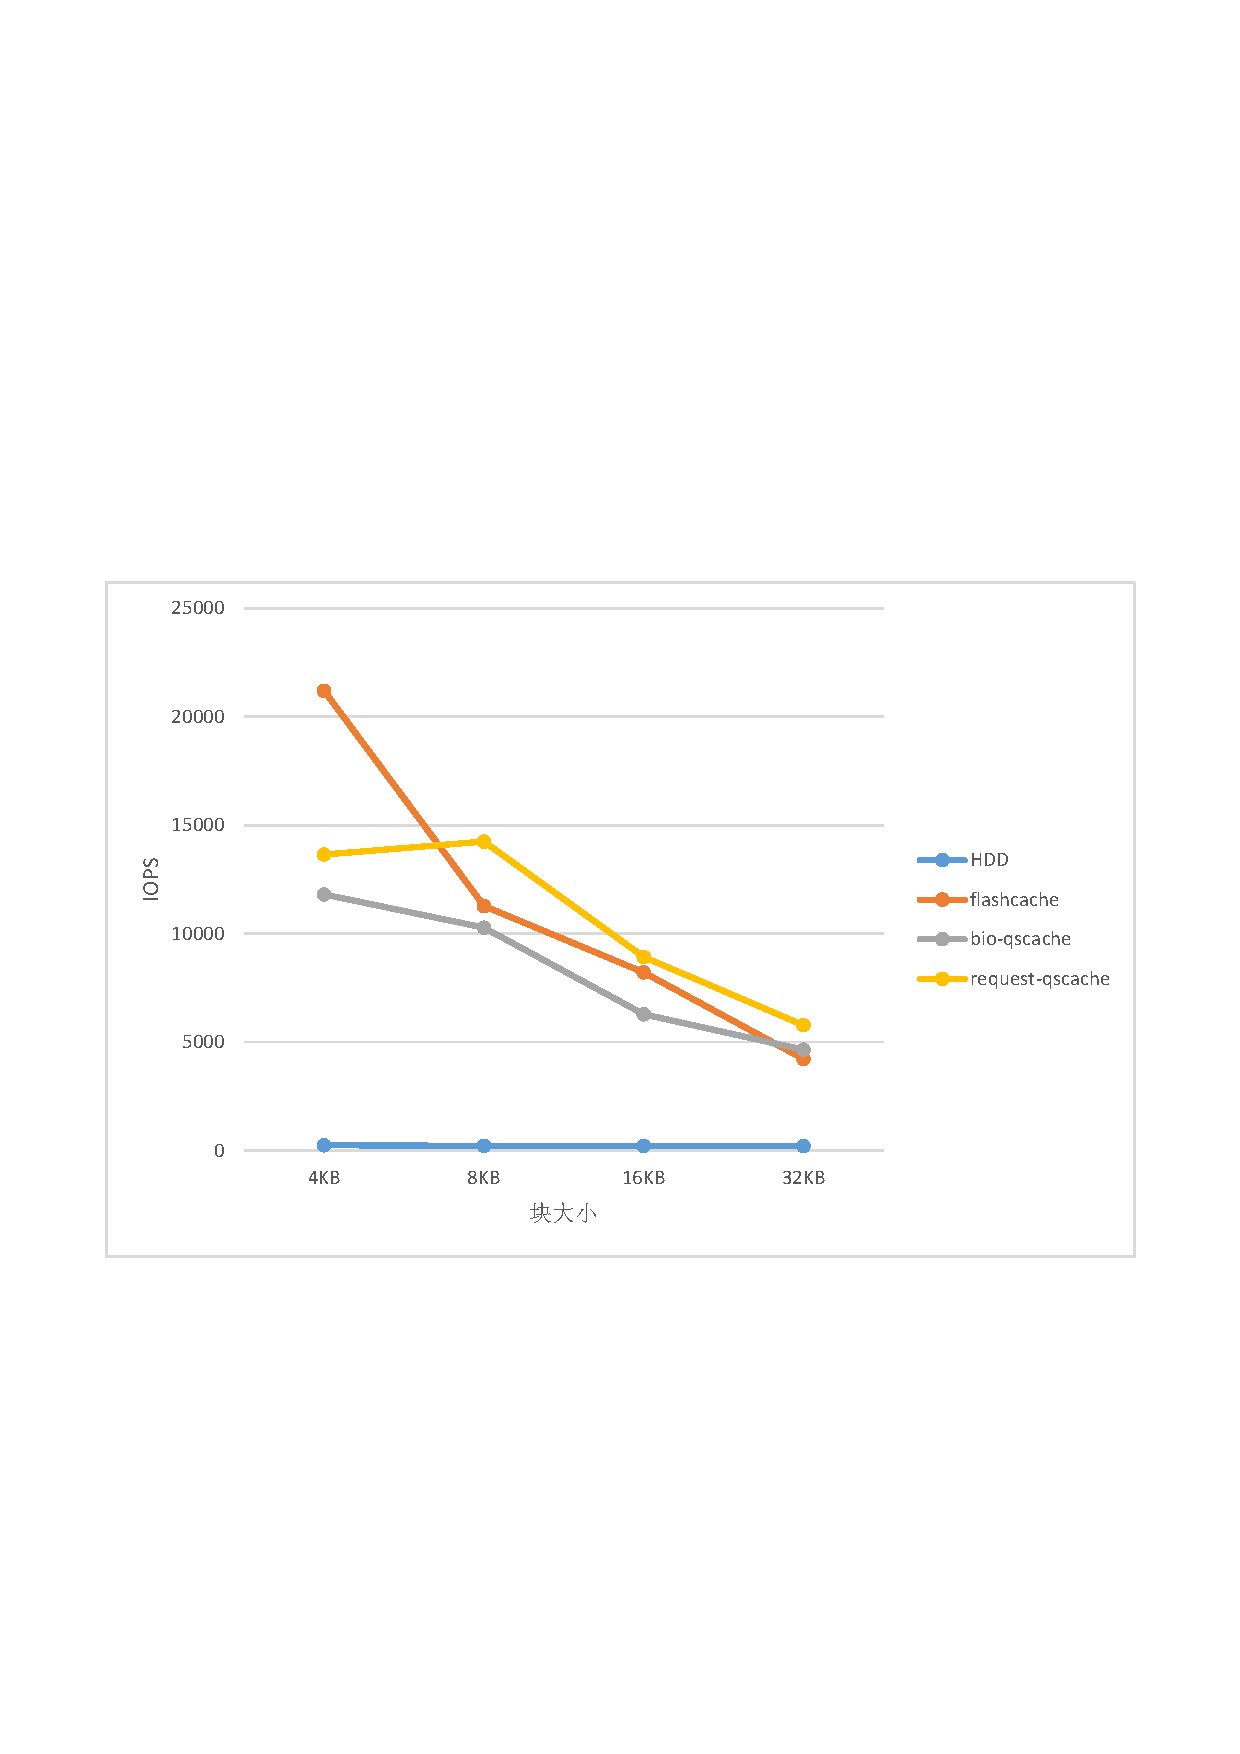
\includegraphics[width=0.8\textwidth]{rand_read.pdf}
    \bicaption[fig:rand_read_comparison]{HDD、flashcache、qscache随机读性能对比图}{HDD、flashcache、qscache随机读性能对比图}{Fig.}{comparison of random read among HDD, flashcache and qscache}
\end{figure}

\begin{figure}[!htbp]
    \centering
    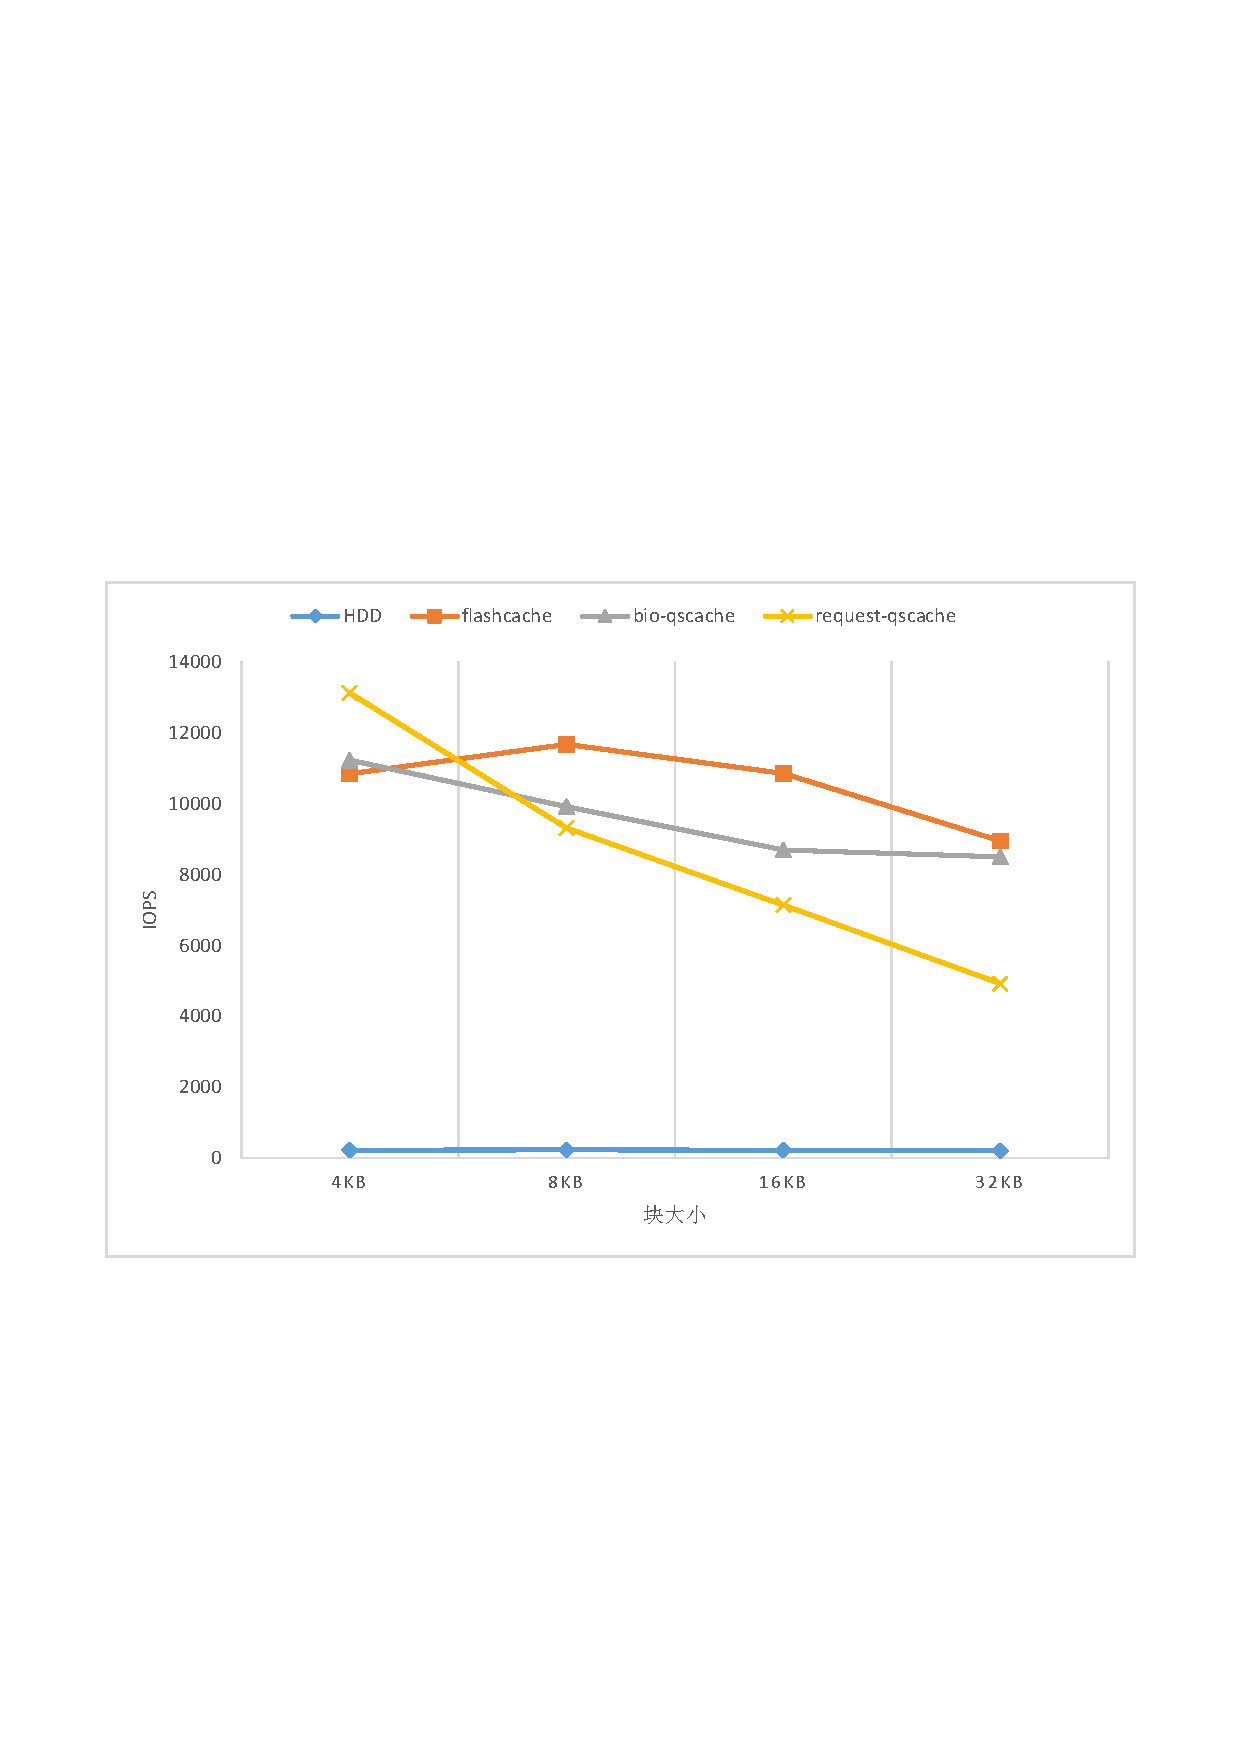
\includegraphics[width=0.8\textwidth]{rand_write.pdf}
    \bicaption[fig:rand_write_comparison]{HDD、flashcache、qscache随机写性能对比图}{HDD、flashcache、qscache随机写性能对比图}{Fig.}{comparison of random write among HDD, flashcache and qscache}
\end{figure}

\subsection{测试分析}

从测试结果来看,在顺序读写性能方面,qscache系统仍无法达到HDD的水平,由于qscache系统整体设计基于flashcache,因此性能大致与flashcache接近,另外可以发现不论是基于bio还是基于request,qscache系统的顺序读写性能也基本接近,这是由于对于顺序读写,系统会进行判断,将大部分顺序请求过滤不进行缓存,因此最后都会实际落到HDD上进行操作,而对HDD而言,本身会延缓执行,等待一小段时间,然后将请求排序再执行,因此即便是基于request的模式,将bio生成request相对而言的额外时间开销对系统影响不大。在随机读写性能方面,qscache系统远超HDD的性能,可见将SSD作为缓存很好地发挥了作用。在随机读时,性能整体能达到flashcache的水平,而在随机写时,基于bio的模式仍能大致维持flashcache的性能,但基于request的模式性能随着I/O块的增大急剧衰减,推测是由于I/O的增大,将bio生成request的过程也会相应消耗更多时间,导致系统整体性能下降。

\section{I/O带宽按权限分配测试}

\subsection{系统初始化}
qscache以基于request的模式启动,初始化操作如下:
\begin{enumerate}
    \item 编译,需要内核的源码树:make KERNEL\_TREE=/usr/src/linux-3.10.108/
    \item 加载,以基于request的模式加载:insmod src/qscache.ko request\_based=1
    \item 以写回模式创建混合存储系统,缓存设备容量120GB,后台设备容量1TB,mapped device命名为cachedev:qscache\_create -p back -n cachedev -c /dev/sdb -h /dev/sdi
    \item I/O scheduler使用cfq:echo cfq > /sys/block/dm-2/queue/scheduler
\end{enumerate}

对I/O带宽按权限分配的测试采用fio工具,通过设置fio的不同group的cgroup的weight设置不同测试进程的权限值并测试他们对系统的mapped device的读写性能是否按照权限进行分配。测试结果如表\ref{tab:qscache_io_test}所示,分多组测试,每组测试的cgroup的weight分别设置不同值,可以看到每组测试中I/O带宽按照权重分配了。

\begin{table}[!hpb]
    \centering
    \bicaption[tab:qscache_io_test]{qscacheI/O带宽按权限分配测试}{qscacheI/O带宽按权限分配测试}{Table}{qscache I/O quota test}
    \begin{tabular}{@{}cccccccccc@{}} 
        \toprule
        \multicolumn{5}{c}{weight} & \multicolumn{5}{c}{IOPS}\\
        group1 & group2 & group3 & group4 & group5 & group1 & group2 & group3 & group4 & group5 \\
        \midrule
        1000 & 800 & 600 & 400 & 0 & 18962 & 15757 & 12263 & 8300 & 0\\
        1000 & 400 & 200 & 100 & 0 & 15785 & 7646 & 3906 & 2007 & 0 \\ 
        500 & 500 & 500 & 500 & 0 & 11685 & 11775 & 11230 & 11055 & 0 \\ 
        1000 & 800 & 400 & 200 & 100 & 22205 & 19052 & 10094 & 5028 & 2400\\ 
        100 & 200 & 300 & 400 & 500 & 3390 & 6699 & 10435 & 13924 & 16652\\
        \bottomrule
    \end{tabular}
\end{table}

\section{qscache的多缓存设备对多后台设备}

多缓存设备对多后台设备的测试环境为仿真环境,在虚拟机中添加多块SSD盘与多块HDD盘进行测试,容量设置为4块1G大小的SSD、2块2G大小的SSD、1块4G大小的SSD以及2块10G大小的HDD与1块20G大小的HDD。1G的SSD为/dev/sdb、/dev/sdc、/dev/sdd、/dev/sde,2G的SSD为/dev/sdf、/dev/sdg,4G的SSD为/dev/sdh,10G的HDD为/dev/sdi、/dev/sdj,20G的HDD/dev/sdk。在系统初始化时分别设置缓存设备为sdh、sdf+sdg、sdb+sdc+sdd+sde,后台设备分别为sdk、sdi+sdj,然后启动系统,测试发现系统都能正常启动,且能正常读写。

\section{本章小结}

本章介绍了qscache系统的测试,首先介绍了系统的测试目标与测试方法,给出了测试环境,然后给出了内核的修改过程和各系统的初始化过程,之后针对各系统测试了顺序读写性能和随机性能,结果显示qscache系统的性能整体与flashcache相近。然后测试了qscache系统对于I/O带宽按权限分配的功能,测试分为几组,每组内进程权限分配不同,结果显示qscache系统成功按不同权限分配了不同的IOPS实现了I/O带宽的按权限分配。最后在仿真环境中测试发现qscache成功实现多缓存设备对多后台设备的功能。